\documentclass[11pt, a4paper]{article}

% ── Packages ──────────────────────────────────────────────────────────────────
\usepackage[margin=1in]{geometry}
\usepackage{amsmath, amssymb}
\usepackage{booktabs}
\usepackage{graphicx}
\usepackage{caption}
\usepackage{subcaption}
\usepackage{float}
\usepackage{hyperref}
\usepackage{xcolor}
\usepackage{enumitem}
\usepackage{array}
\usepackage{multirow}
\usepackage{tabularx}
\usepackage{setspace}
\usepackage{parskip}
\usepackage{microtype}
\usepackage{fancyhdr}
\usepackage{titlesec}
\usepackage{natbib}

% ── Hyperref setup ─────────────────────────────────────────────────────────────
\hypersetup{
  colorlinks = true,
  linkcolor  = blue!70!black,
  citecolor  = blue!70!black,
  urlcolor   = blue!70!black
}

% ── Header / footer ───────────────────────────────────────────────────────────
\pagestyle{fancy}
\fancyhf{}
\rhead{\small STAT GR5243 --- Spring 2026}
\lhead{\small Group 20 --- A/B Test Report}
\rfoot{\thepage}
\renewcommand{\headrulewidth}{0.4pt}

% ── Section title formatting ──────────────────────────────────────────────────
\titleformat{\section}{\large\bfseries}{\thesection.}{0.5em}{}[\titlerule]
\titleformat{\subsection}{\normalsize\bfseries}{\thesubsection}{0.5em}{}

% ── Spacing ───────────────────────────────────────────────────────────────────
\setlength{\parskip}{6pt}
\setlength{\parindent}{0pt}
\onehalfspacing

% ── Column type for tables ────────────────────────────────────────────────────
\newcolumntype{L}[1]{>{\raggedright\arraybackslash}p{#1}}
\newcolumntype{C}[1]{>{\centering\arraybackslash}p{#1}}
\newcolumntype{R}[1]{>{\raggedleft\arraybackslash}p{#1}}

% =============================================================================
\begin{document}
% =============================================================================

% ── Title ─────────────────────────────────────────────────────────────────────
\begin{titlepage}
  \centering
  \vspace*{2cm}
  {\LARGE\bfseries Does Guided Onboarding Improve Task Completion\\[6pt]
   in a Data Analysis Interface?\par}
  \vspace{0.4cm}
  {\large An A/B Test\par}
  \vspace{1.5cm}
  {\large STAT GR5243 --- Applied Data Science, Spring 2026\par}
  \vspace{0.5cm}
  {\normalsize\textbf{Group 20}\par}
  \vspace{0.3cm}
  {\normalsize
    Duoli Chen (dc3940) \quad Ketaki Dabade (kvd2112) \\[4pt]
    Yueyou Tao (yt2995) \quad Pin Wang (pw2661)\par}
  \vspace{0.8cm}
  {\normalsize
    Repository: \href{https://github.com/yt2995-lucia/project-3-applied-ver}
                     {github.com/yt2995-lucia/project-3-applied-ver}\par}
  \vfill
  {\normalsize \today\par}
\end{titlepage}

% ── Abstract ──────────────────────────────────────────────────────────────────
\begin{abstract}
\noindent
We present a between-subject A/B test investigating whether step-by-step onboarding
hints improve task completion in a web-based data analysis interface. Participants
were randomly assigned to either an unguided control (Group~A, $n=52$) or a guided
treatment (Group~B, $n=45$) in a custom R Shiny application. The primary outcome was
full completion of five sequential data tasks. Group~B achieved a 71.1\% completion
rate versus 42.3\% in Group~A ($\chi^2(1)=6.985$, $p=0.0082$, Cram\'er's $V=0.268$;
Fisher's OR$_{\text{B vs A}}=3.36$, 95\%~CI: [1.44, 7.82]). Time-per-task among
completers was non-significantly longer in Group~B (median 17.0s vs.\ 8.1s,
Mann--Whitney $p=0.096$). Results were robust to outlier removal. Subgroup analysis
revealed that hints benefited experienced users substantially (Fisher $p=0.003$) but
not inexperienced users ($p=1.0$). We conclude that guided onboarding meaningfully
improves task success with a modest, non-significant time cost.
\end{abstract}

\tableofcontents
\newpage

% =============================================================================
\section{Introduction \& Research Question}
% =============================================================================

As data analysis tools become increasingly accessible to non-expert users, interface
design plays a critical role in whether users can effectively complete analytical
tasks. Poor onboarding --- or the complete absence of guidance --- may lead users to
abandon tasks prematurely, reducing the practical utility of even well-built tools.

This study investigates the following research question:

\begin{quote}
\textit{Does providing step-by-step instructional guidance in a data analysis
interface improve task completion rate compared to an unguided interface?}
\end{quote}

We hypothesize that users who receive explicit hints and reasoning at each task step
(treatment group) will complete significantly more tasks than users who must explore
the interface independently (control group):

\begin{itemize}[leftmargin=1.5em]
  \item \textbf{H\textsubscript{0}:} No difference in task completion rate or time
        efficiency between Group~A (no hints) and Group~B (hints).
  \item \textbf{H\textsubscript{1}:} Group~B achieves a significantly higher task
        completion rate than Group~A.
\end{itemize}

% =============================================================================
\section{Experimental Design \& Methodology}
% =============================================================================

We conducted a between-subject A/B test using a custom-built R Shiny application
called \textit{DataScope}, which presents participants with five sequential data
analysis tasks on the \texttt{iris} dataset (with 19 artificially injected missing
values across two columns).

\subsection{Group Conditions}

\begin{itemize}[leftmargin=1.5em]
  \item \textbf{Group~A (Control):} Participants received vague task descriptions
        and no guidance, requiring independent exploration of the interface.
  \item \textbf{Group~B (Treatment):} Participants received the same tasks
        accompanied by explicit step-by-step hints explaining both \emph{what} to
        do and \emph{why}, along with pop-up notifications directing them to the
        next task upon completion.
\end{itemize}

Group assignment was randomized at session initiation using a Bernoulli draw
(\texttt{runif(1) > 0.5}), ensuring approximately equal allocation. Each
participant completed the study independently with no time limit.

\subsection{Task Definitions}

Table~\ref{tab:tasks} shows the five tasks as presented to each group.

\begin{table}[H]
\centering
\caption{Task descriptions by condition.}
\label{tab:tasks}
\begin{tabularx}{\textwidth}{c L{5.5cm} L{6cm}}
\toprule
\textbf{Task} & \textbf{Group A (vague description)} & \textbf{Group B (explicit instruction)} \\
\midrule
1 & Explore the loaded data
  & Browse the first 10 rows of the pre-loaded dataset \\
\addlinespace
2 & Understand the basic properties of each column
  & Click \textit{Generate Summary} to produce summary statistics for all columns \\
\addlinespace
3 & Remove the non-numerical column from the dataset
  & Select \textit{Species} from the dropdown and click \textit{Remove Column} \\
\addlinespace
4 & Create a histogram of the variable with the highest mean value
  & Select \textit{Sepal.Length} (highest mean $\approx$ 5.84) and click \textit{Create Histogram} \\
\addlinespace
5 & Check the data quality of the dataset
  & Click \textit{Check Missing Values} to identify columns with missing entries \\
\bottomrule
\end{tabularx}
\end{table}

\subsection{Metrics}

\begin{itemize}[leftmargin=1.5em]
  \item \textbf{Primary:} Task completion rate --- proportion of participants who
        successfully completed all five tasks ($n\_tasks\_done = 5$).
  \item \textbf{Secondary:} Total session time (seconds), per-task completion
        rates, average time per completed task (seconds), and self-reported
        perceived difficulty.
\end{itemize}

% =============================================================================
\section{Data Collection}
% =============================================================================

Data were collected automatically via the Shiny application and logged to Google
Sheets through a Google Apps Script web endpoint. Each submission captured:
session ID, participant ID, group assignment, number of tasks completed (0--5),
total session time (seconds), per-task completion status (\texttt{TRUE}/\texttt{FALSE}),
cumulative elapsed time to each completed task, self-reported prior data experience
(Yes/No), and perceived task difficulty (Yes/No).

Participants were recruited through personal networks, classmates, and social media
sharing of the app URL. A total of 97 submissions were collected, assigned unique
participant IDs P001--P097. Some participants restarted the app and submitted multiple
times under different session IDs; each submission is treated as an independent
observation consistent with the between-subject design, as each reflects a distinct
randomized interaction with the interface.

After cleaning (see \texttt{data\_cleaning.py}), the final dataset comprises 97
records: Group~A ($n=52$) and Group~B ($n=45$). One participant (P086) did not
complete the post-task survey, resulting in missing values for the experience and
difficulty covariates; this record is included in the primary completion-rate
analysis but excluded from covariate subgroup analyses.

The cleaned dataset was exported to \texttt{ab\_test\_clean\_keep\_outliers.csv}
(all 97 valid records) and \texttt{ab\_test\_clean\_no\_outliers.csv} (93 records
after IQR-based removal of extreme session times), used for the primary and
sensitivity analyses respectively.

% =============================================================================
\section{Statistical Analysis \& Results}
% =============================================================================

\subsection{Analytical Approach}

All analyses were conducted in Python using \texttt{pandas}, \texttt{scipy},
\texttt{statsmodels}, \texttt{matplotlib}, and \texttt{seaborn}. The primary
outcome (binary: completed all 5 tasks) was analyzed with chi-square and
Fisher's exact tests. The secondary outcome (continuous: average time per
completed task) was first assessed for normality using Shapiro--Wilk tests;
all variables were non-normal in both groups ($p < 0.0001$), so Mann--Whitney~$U$
was the primary test for continuous comparisons. Welch's $t$-test and a
10{,}000-iteration percentile bootstrap are reported as supplementary checks.
Effect sizes (Cram\'er's~$V$, rank-biserial~$r$, Cohen's~$d$ and $h$) and 95\%
confidence intervals are provided for all primary tests. A sensitivity analysis
repeats all tests on the trimmed dataset ($n=93$).

\subsection{Descriptive Statistics}

Table~\ref{tab:desc} summarises the key outcome variables by group.

\begin{table}[H]
\centering
\caption{Descriptive statistics by group (full dataset, $n=97$).}
\label{tab:desc}
\begin{tabular}{lcc}
\toprule
\textbf{Metric} & \textbf{Group A (No Hints, $n=52$)} & \textbf{Group B (Hints, $n=45$)} \\
\midrule
Completed all 5 tasks & 22 (42.3\%) & 32 (71.1\%) \\
Median tasks completed & 4.0 & 5.0 \\
Mean tasks completed (SD) & 3.44 (1.70) & 4.36 (1.28) \\
Mean total session time, s (SD) & 69.1 (74.8) & 113.0 (104.9) \\
Median total session time, s & 40.5 & 66.0 \\
Mean avg.\ time/task, completers (SD) & 16.2s (17.6) & 23.8s (20.9) \\
Median avg.\ time/task, completers & 8.1s & 17.0s \\
\bottomrule
\end{tabular}
\end{table}

Group~B participants completed substantially more tasks (median = 5 vs.\ 4) and
had a 28.8 percentage-point higher full-completion rate. Among completers, Group~A
was faster per task (median 8.1s vs.\ 17.0s), reflecting the time Group~B spent
reading hint text.

Figure~\ref{fig:completion} shows the completion rate stacked bar chart and the
distribution of tasks completed per participant. Figure~\ref{fig:time} shows
boxplots of average time per task (completers only) and kernel density estimates
of total session time.

\begin{figure}[H]
  \centering
  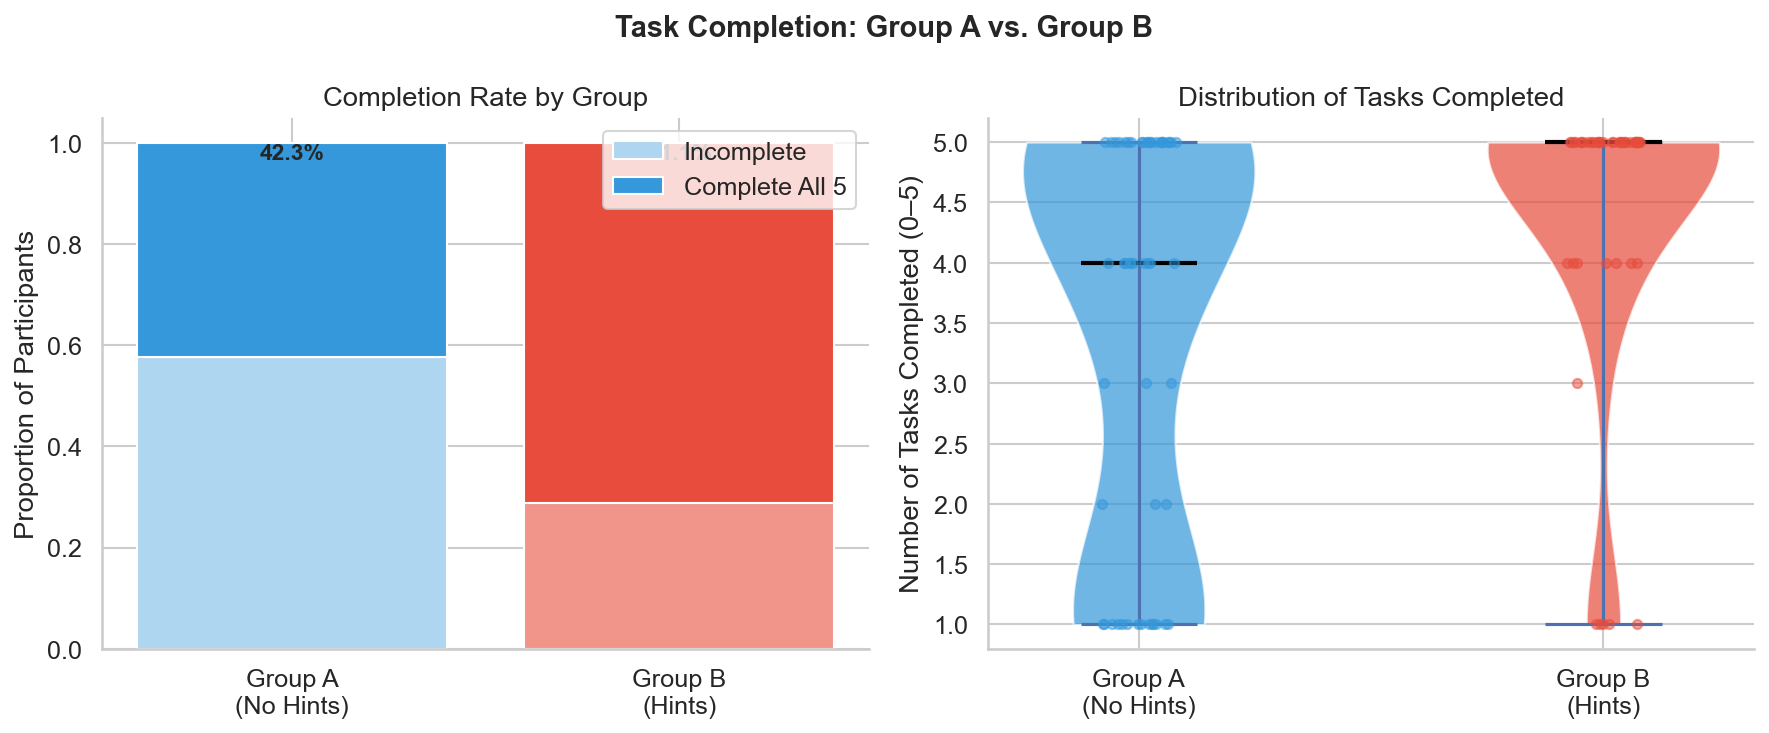
\includegraphics[width=0.95\textwidth]{figures/fig1_completion.png}
  \caption{Left: proportion of participants who completed all five tasks by group
           (dark fill = complete, light fill = incomplete), with completion
           percentages annotated. Right: violin plot with individual observations
           (jittered) of tasks completed (0--5) per participant.}
  \label{fig:completion}
\end{figure}

\begin{figure}[H]
  \centering
  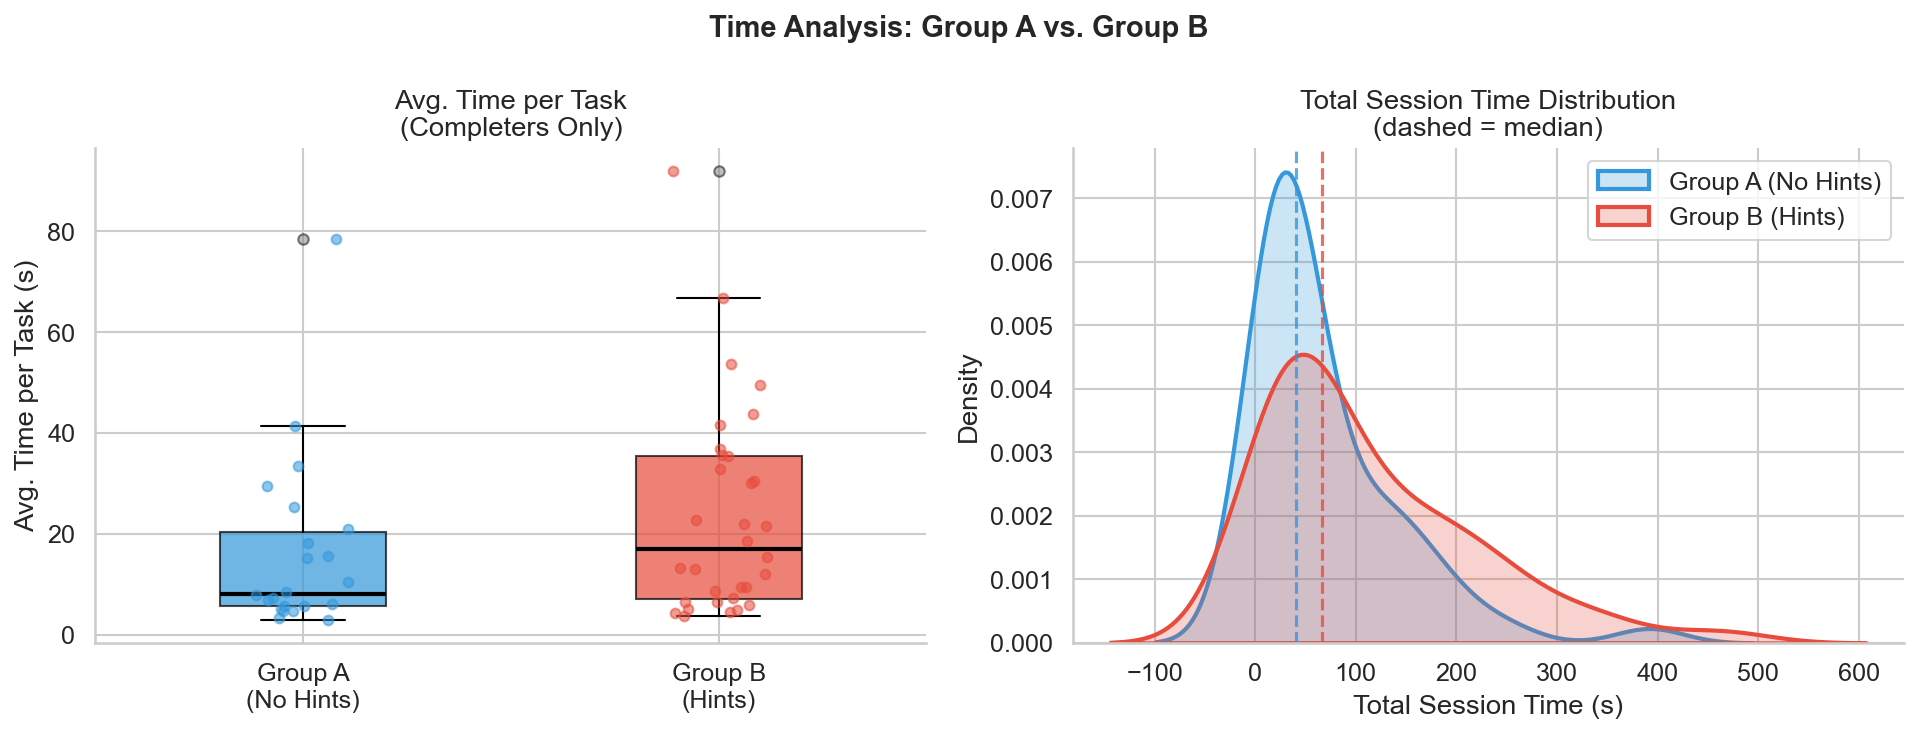
\includegraphics[width=0.95\textwidth]{figures/fig2_time.png}
  \caption{Left: box-and-strip plot of average time per completed task for
           participants who finished all five tasks. Right: kernel density estimates
           of total session time for all participants (dashed lines = group medians).}
  \label{fig:time}
\end{figure}

\subsection{Primary Analysis: Task Completion Rate}

Three concordant tests were applied to the binary completion outcome
(Table~\ref{tab:primary}).

\begin{table}[H]
\centering
\caption{Primary analysis --- task completion rate (binary outcome).}
\label{tab:primary}
\begin{tabular}{lccc}
\toprule
\textbf{Test} & \textbf{Statistic} & \textbf{$p$-value} & \textbf{Effect size} \\
\midrule
Chi-square ($\chi^2$, $df=1$) & $\chi^2 = 6.985$ & \textbf{0.0082} & Cram\'er's $V = 0.268$ \\
Fisher's Exact Test            & OR$_{\text{B vs A}} = 3.36$ & \textbf{0.0074} & 95\% CI: [1.44, 7.82] \\
Two-proportion $z$-test        & $z = 2.848$ & \textbf{0.0044} & Cohen's $h = 0.590$ \\
Mann--Whitney $U$ (task count) & $U = 799.5$ & \textbf{0.0030} & $r = 0.317$ \\
\bottomrule
\end{tabular}
\end{table}

All three tests consistently reject H\textsubscript{0} at $\alpha = 0.05$. Group~B
participants had 3.36 times the odds of completing all tasks compared to Group~A
(Fisher's OR$_{\text{B vs A}} = 3.36$, 95\% CI: [1.44, 7.82]). Cohen's $h = 0.590$
and Cram\'er's $V = 0.268$ indicate a small-to-medium effect size. A Mann--Whitney
$U$ test on the raw task count (0--5) confirmed the same direction ($p = 0.003$,
rank-biserial $r = 0.317$).

\textbf{Per-task completion rates} (Figure~\ref{fig:pertask}) reveal where
divergence occurred. Both groups completed Task~1 at 100\% (auto-marked on tab
visit). The gap widened progressively and peaked at Task~4 --- creating a histogram
of the highest-mean variable --- where Group~A dropped to 44.2\% versus 73.3\% in
Group~B. This was the most cognitively demanding task, requiring independent
identification of \textit{Sepal.Length} as the target column.

\begin{table}[H]
\centering
\caption{Per-task completion rates by group.}
\label{tab:pertask}
\begin{tabular}{lccr}
\toprule
\textbf{Task} & \textbf{Group A} & \textbf{Group B} & \textbf{Difference} \\
\midrule
Task 1: View data          & 100.0\% & 100.0\% & $+$0.0 pp \\
Task 2: Summary statistics &  73.1\% &  88.9\% & $+$15.8 pp \\
Task 3: Remove column      &  61.5\% &  86.7\% & $+$25.2 pp \\
Task 4: Histogram          &  44.2\% &  73.3\% & $+$29.1 pp \\
Task 5: Missing values     &  65.4\% &  86.7\% & $+$21.3 pp \\
\bottomrule
\end{tabular}
\end{table}

\begin{figure}[H]
  \centering
  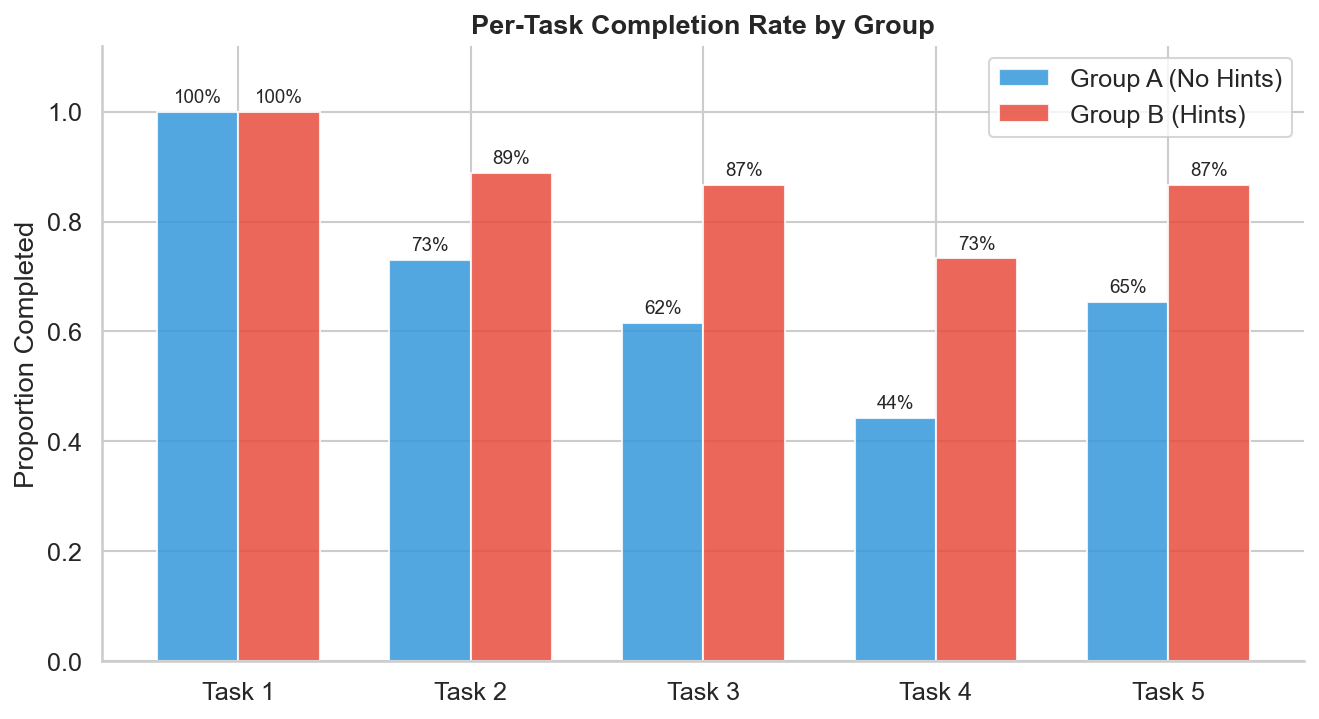
\includegraphics[width=0.80\textwidth]{figures/fig3_per_task.png}
  \caption{Per-task completion rates by group. The largest gap occurs at Task~4
           (histogram), which required identifying the highest-mean column
           independently in Group~A.}
  \label{fig:pertask}
\end{figure}

\subsection{Secondary Analysis: Time Efficiency}

Time comparisons were restricted to participants who completed all five tasks
($n_A = 22$, $n_B = 32$) to avoid confounding by partial completion.

\begin{table}[H]
\centering
\caption{Secondary analysis --- average time per completed task (completers only).}
\label{tab:time}
\begin{tabular}{lccc}
\toprule
\textbf{Test} & \textbf{Statistic} & \textbf{$p$-value} & \textbf{Effect size} \\
\midrule
Mann--Whitney $U$ (avg time/task)   & $U = 257.0$ & 0.0961 & $r = 0.270$ \\
Welch's $t$-test (avg time/task)    & $t = -1.450$ & 0.1534 & Cohen's $d = -0.389$ \\
Bootstrap 95\% CI (mean diff, A$-$B) & $\Delta = -7.64$s & --- & [$-$17.46, $+$3.03] \\
\bottomrule
\end{tabular}
\end{table}

Group~A completers were faster per task (mean 16.2s vs.\ 23.8s; median 8.1s
vs.\ 17.0s), but the difference did not reach statistical significance
(MWU $p = 0.096$). The bootstrap 95\% CI for the mean difference (A$-$B) spans
zero [$-$17.46, $+$3.03], confirming this null result. The small-to-medium
point estimate ($d = -0.389$) combined with the non-significant $p$-value reflects
low post-hoc power (28\%) in the completers-only subsample, so a time tradeoff
cannot be definitively ruled out.

For total session time across \emph{all} participants, Group~B spent significantly
more time overall (median 66.0s vs.\ 40.5s; MWU $U = 835.0$, $p = 0.0155$,
$r = 0.286$), reflecting the additional time reading hints and following navigation
prompts.

Figure~\ref{fig:cumutime} shows the cumulative elapsed time at each task
completion milestone, capturing how the two groups progressed through the five
tasks over time.

\begin{figure}[H]
  \centering
  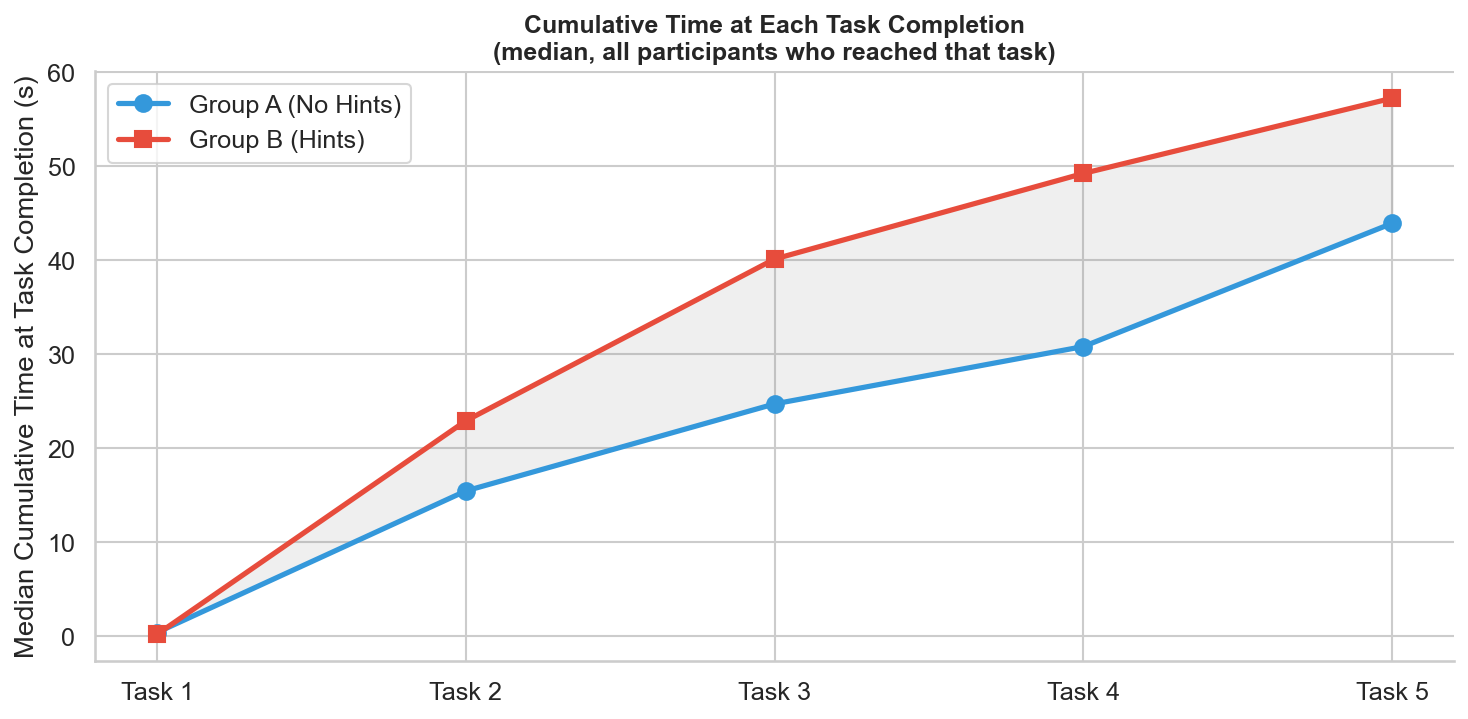
\includegraphics[width=0.75\textwidth]{figures/fig4_per_task_time.png}
  \caption{Median cumulative elapsed time (seconds from session start) at each
           task completion milestone, for participants who reached that task.
           Group~B accumulates more time at every step, consistent with hint-reading
           overhead.}
  \label{fig:cumutime}
\end{figure}

\subsection{Subgroup Analysis}

To examine whether the hint effect was moderated by participant characteristics,
Fisher's exact tests were conducted within strata of prior experience and perceived
difficulty (Figure~\ref{fig:subgroup}).

\begin{table}[H]
\centering
\caption{Subgroup analysis --- task completion by prior experience.}
\label{tab:subgroup}
\begin{tabular}{lccccc}
\toprule
\textbf{Subgroup} & \textbf{$n$} & \textbf{Group A} & \textbf{Group B}
  & \textbf{OR (B vs A)} & \textbf{$p$ (Fisher)} \\
\midrule
Experienced (Yes) & 66 & 12/33 = 36.4\% & 25/33 = 75.8\% & 5.56 & \textbf{0.003} \\
Inexperienced (No) & 30 & 10/18 = 55.6\% & 7/12 = 58.3\%  & 1.12 & 1.000 \\
\midrule
Found tasks difficult (Yes) & 62 & 15/39 = 38.5\% & 14/23 = 60.9\% & 2.49 & 0.116 \\
Did not find tasks difficult (No) & 34 & 7/12 = 58.3\% & 18/22 = 81.8\% & 3.21 & 0.224 \\
\bottomrule
\end{tabular}
\end{table}

The hint effect was concentrated entirely among users with prior data analysis
experience ($p = 0.003$; OR = 5.56), while no significant difference appeared among
inexperienced users ($p = 1.0$). This suggests that experienced users could leverage
the hints effectively --- they possessed the conceptual vocabulary needed to act on
the guidance --- whereas inexperienced users faced a base difficulty level that
hints alone were insufficient to overcome. Subgroup results for perceived difficulty
were directionally consistent but did not reach significance individually, likely
due to reduced subsample sizes.

\begin{figure}[H]
  \centering
  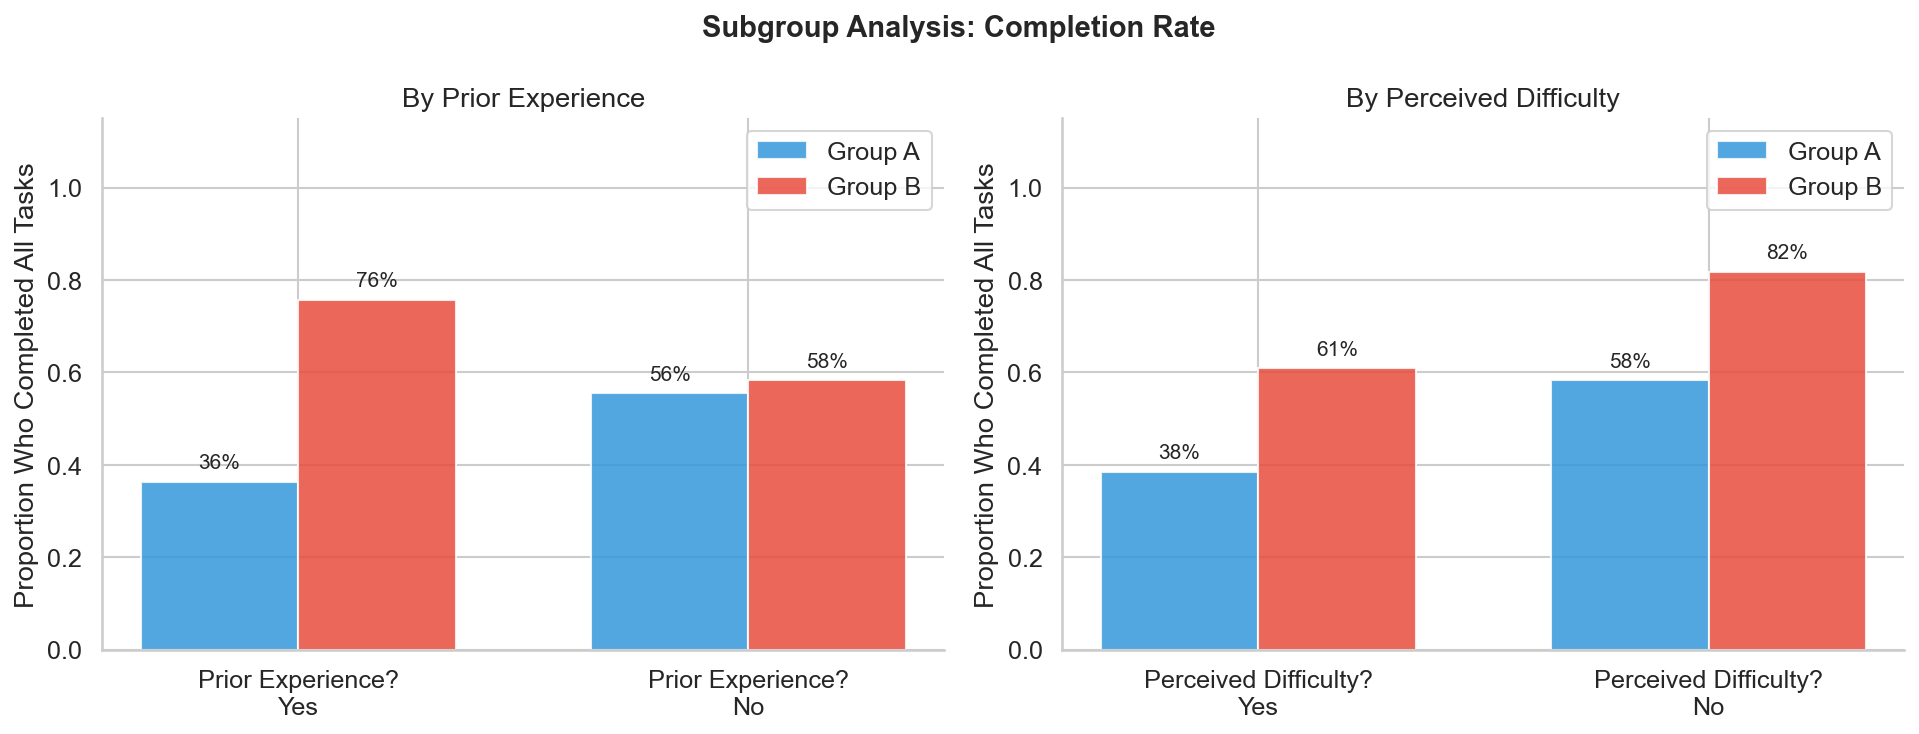
\includegraphics[width=0.90\textwidth]{figures/fig5_subgroup.png}
  \caption{Task completion rates by group, stratified by prior experience (left)
           and perceived difficulty (right).}
  \label{fig:subgroup}
\end{figure}

\subsection{Sensitivity Analysis}

Repeating all primary tests on the outlier-trimmed dataset ($n=93$, IQR-based
time outlier removal) yielded consistent results:
$\chi^2(1)=7.334$, $p=0.0068$, Cram\'er's $V=0.281$ for completion; MWU $p=0.090$
for time among completers. The primary conclusion is robust to the presence or
absence of high-time outliers.

\subsection{Post-Hoc Power Analysis}

The chi-square test for completion was well-powered: post-hoc power $\approx 1.00$
at $\alpha = 0.05$, $n = 97$, with observed Cohen's $h = 0.590$. By contrast, the
time test among completers was underpowered (post-hoc power = 28\% at
$\alpha = 0.05$, $n_A = 22$, $n_B = 32$, $d = 0.389$), indicating that a larger
completers-only sample would be needed to reliably detect a time effect of this
magnitude.

\begin{figure}[H]
  \centering
  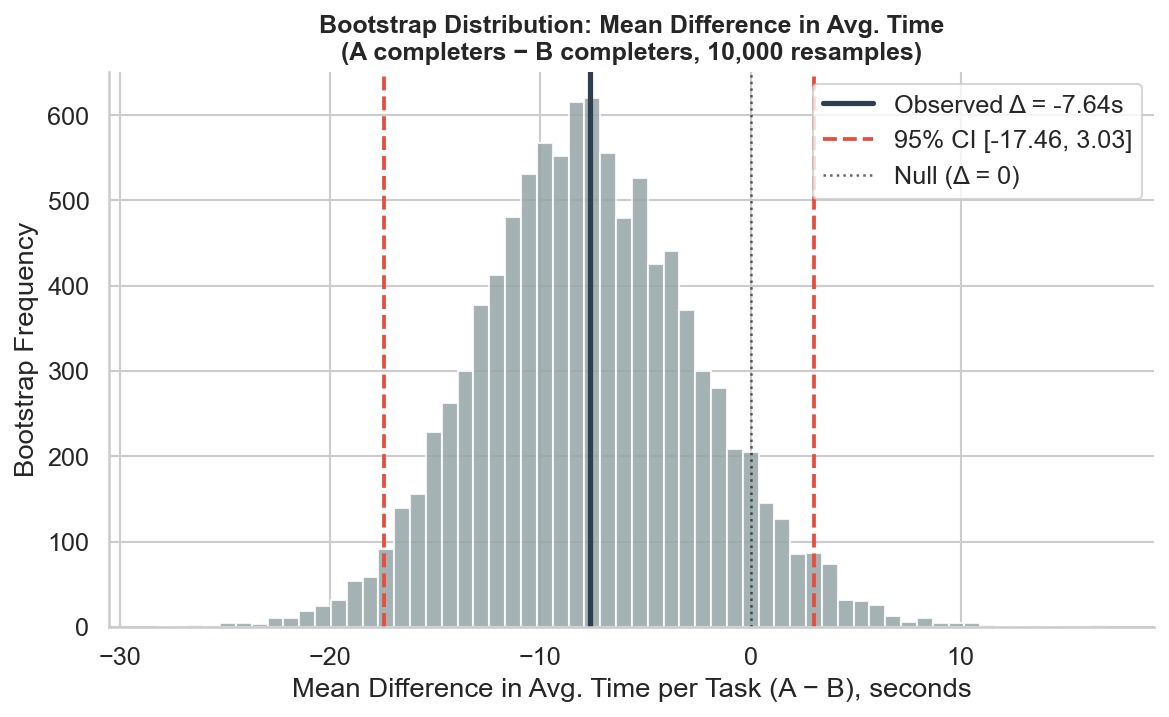
\includegraphics[width=0.72\textwidth]{figures/fig6_bootstrap.png}
  \caption{Bootstrap sampling distribution (10{,}000 resamples) of the mean
           difference in average time per task (Group~A $-$ Group~B, completers
           only). The 95\% CI [$-$17.46, $+$3.03] crosses zero, consistent with
           a non-significant time difference.}
  \label{fig:bootstrap}
\end{figure}

% =============================================================================
\section{Interpretation \& Conclusion}
% =============================================================================

The experiment provides consistent, statistically significant evidence that
step-by-step onboarding guidance (Group~B) improves task completion in a data
analysis interface. We reject H\textsubscript{0} for the primary outcome:
Group~B participants completed all five tasks at a rate 28.8 percentage points
higher than Group~A (71.1\% vs.\ 42.3\%; $\chi^2(1)=6.985$, $p=0.0082$;
Fisher's OR$_{\text{B vs A}}=3.36$). This effect held across all statistical
approaches and was robust to outlier removal.

The secondary time analysis reveals an important tradeoff: among users who
completed all tasks, guided participants (Group~B) took longer per task (median
17.0s vs.\ 8.1s), though this difference was not statistically significant
($p = 0.096$). Rather than indicating inefficiency, this likely reflects the
time participants spent reading the step-by-step hint boxes --- an expected cost
of guidance-driven interfaces. Group~A completers, necessarily a self-selected
subset of more capable or determined users, navigated the interface faster;
however, 57.7\% of Group~A never reached full completion at all.

The subgroup analysis adds a nuanced finding: hints provided the largest benefit
to users with prior data experience (OR = 5.56, $p = 0.003$), while inexperienced
users completed tasks at nearly equal rates regardless of condition ($\sim$56\% vs.\
$\sim$58\%, $p = 1.0$). This suggests that hint-based guidance is a necessary but
insufficient condition for supporting true novices --- deeper scaffolding such as
interactive tutorials or worked examples may be required for users who lack
foundational data literacy.

\textbf{Practical recommendation:} Guided onboarding (step-by-step hints with
navigation prompts) should be the default interface for data analysis tools
targeting mixed-expertise audiences. The completion benefit is substantial and
statistically robust (effect size $h = 0.590$). The time cost is modest and
non-significant, and represents an acceptable tradeoff for a 28.8 percentage-point
improvement in task success.

% =============================================================================
\section{Challenges \& Limitations}
% =============================================================================

\textbf{Sample size and power.}
The study collected 97 submissions from a convenience sample. While sufficient to
detect the completion-rate effect with high power ($\approx 1.00$), the time
comparison among completers only ($n = 54$) was underpowered (28\%), meaning we
cannot firmly conclude the time difference is zero --- only that the current data
do not support rejecting H\textsubscript{0} for time. A future study targeting
$n \approx 100$ completers per group would have $> 80\%$ power to detect an effect
of $d = 0.389$.

\textbf{Convenience sampling and selection bias.}
Participants were recruited through personal networks and social media; the sample
is likely dominated by students with some quantitative background. The subgroup
analysis already suggests this limits generalizability to true novices, for whom
the hint condition showed no benefit.

\textbf{Multiple submissions.}
Several participants submitted more than once under different session IDs (e.g.,
restarting the app). We treated each submission as an independent observation
consistent with the between-subject design. However, learning effects across
repeated attempts may have slightly inflated completion rates for repeat
participants in both groups.

\textbf{Confounded treatment components.}
Group~B received not only informational hints but also pop-up navigation
notifications directing them to the next task after each completion. It is therefore
impossible to isolate whether the improvement came from the hint content, the
navigational prompts, or their combination. A three-arm design
(A: no hints, no prompts; B: hints only; C: prompts only) would disentangle these
mechanisms.

\textbf{Single dataset and fixed task structure.}
All participants analysed the same \texttt{iris} dataset with identical tasks.
Results may not generalise to other datasets, task structures, or application
domains. Future work should vary dataset complexity and hint specificity to assess
whether a lighter-weight nudge achieves comparable completion gains with less time
overhead.

\textbf{Device and environment heterogeneity.}
The application was accessed remotely on participants' own devices. Screen size,
browser version, internet speed, and ambient distraction were not controlled,
introducing noise into both timing and completion measurements.

% =============================================================================
% Optional: References
% =============================================================================
% \newpage
% \bibliographystyle{plainnat}
% \bibliography{references}

\end{document}
